% !Mode:: "TeX:UTF-8"
\documentclass{article}
% !Mode:: "TeX:UTF-8"
\usepackage[english]{babel}
\usepackage[UTF8]{ctex}
\usepackage{amsmath, amsthm, amssymb}

% Figure
\usepackage{graphicx}
\usepackage{float} %% H can fix the location
\usepackage{caption}
\usepackage[format=hang,singlelinecheck=0,font={sf,small},labelfont=bf]{subfig}
\usepackage[noabbrev]{cleveref}
\captionsetup[subfigure]{subrefformat=simple,labelformat=simple,listofformat=subsimple}
\renewcommand\thesubfigure{(\alph{subfigure})}

\usepackage{epstopdf} %% convert eps to pdf
\DeclareGraphicsExtensions{.eps,.mps,.pdf,.jpg,.png} %% bmp, gif not supported
\DeclareGraphicsRule{*}{eps}{*}{}
\graphicspath{{img/}{figure/}{../figure/}} %% fig directorys

%% \usepackage{pstricks} %% a set of macros that allow the inclusion of PostScript drawings directly inside TeX or LaTeX code
%% \usepackage{wrapfig} %% Wrapping text around figures

% Table
\usepackage{booktabs} %% allow the use of \toprule, \midrule, and \bottomrule
\usepackage{tabularx}
\usepackage{multirow}
\usepackage{colortbl}
\usepackage{longtable}
\usepackage{supertabular}

\usepackage[colorinlistoftodos]{todonotes}

% Geometry
\usepackage[paper=a4paper, top=1.5cm, bottom=1.5cm, left=1cm, right=1cm]{geometry}
%% \usepackage[paper=a4paper, top=2.54cm, bottom=2.54cm, left=3.18cm, right=3.18cm]{geometry} %% ms word
%% \usepackage[top=0.1cm, bottom=0.1cm, left=0.1cm, right=0.1cm, paperwidth=9cm, paperheight=11.7cm]{geometry} %% kindle

% Code
%% \usepackage{alltt} %% \textbf can be used in alltt, but not in verbatim

\usepackage{listings}
\lstset{
    backgroundcolor=\color{white},
    columns=flexible,
    breakatwhitespace=false,
    breaklines=true,
    captionpos=tt,
    frame=single, %% Frame: show a box around, possible values are: none|leftline|topline|bottomline|lines|single|shadowbox
    numbers=left, %% possible values are: left, right, none
    numbersep=5pt,
    showspaces=false,
    showstringspaces=false,
    showtabs=false,
    stepnumber=1, %% interval of lines to display the line number
    rulecolor=\color{black},
    tabsize=2,
    texcl=true,
    title=\lstname,
    escapeinside={\%*}{*)},
    extendedchars=false,
    mathescape=true,
    xleftmargin=3em,
    xrightmargin=3em,
    numberstyle=\color{gray},
    keywordstyle=\color{blue},
    commentstyle=\color{green},
    stringstyle=\color{red},
}

% Reference
%% \bibliographystyle{plain} % reference style

% Color
\usepackage[colorlinks, linkcolor=blue, anchorcolor=red, citecolor=green, CJKbookmarks=true]{hyperref}
\usepackage{color}
\def\red#1{\textcolor[rgb]{1.00,0.00,0.00}{#1}}
\newcommand\warning[1]{\red{#1}}

% Other
%% \usepackage{fixltx2e} %% for use of \textsubscript
%% \usepackage{dirtree}  %% directory structure, like the result of command tree in bash shell


% !Mode:: "TeX:UTF-8"
%+++++++++++++++++++++++++++++++++++article+++++++++++++++++++++++++++++++++
%customize the numbering of equation, to make it like section-subsection-equation style, for example,1-2-3
\makeatletter\@addtoreset{equation}{subsection}\makeatother
\renewcommand\theequation{%
\thepart\arabic{section}%
-\thepart\arabic{subsection}%
-\thepart\arabic{equation}%
}
%theorem
\newtheorem{definition}{D\'efintion} %% 整篇文章的全局编号
\newtheorem*{thmwn}{Thm} %% without numbers
\newtheorem{theorem}{Th\'eor\`eme}[section] %% 从属于section编号
\newtheorem{corollary}{Corollary}[theorem] %% 从属于theorem编号
\newtheorem{lemma}{Lemma}
\newtheorem{proposition}{Proposition}[section]
\newtheorem{example}{Example}
\newtheorem*{attention}{Attention}
\newtheorem*{note}{Note}
\newtheorem*{remark}{Remark}
\newtheorem{question}{Question}[section]
\newtheorem{problem}{Problem}
\newtheorem{fact}{Fact}


% Equation
\newcommand\lasteq{(\theequation)\ } %% use \lasteq to reference the last equation
\newcommand{\eqspace}{\hspace{0.5cm}}
\newcommand{\eqnote}[1]{\text{ #1 }} %% insert text in math mode being treated as normal text
\newcommand\mytop[2]{\genfrac{}{}{0pt}{}{#1}{#2}} %% generate a fraction but without the line

% Vecteur
\def\vecteur#1{(#1_1,~#1_2,~\ldots,~#1_n)}
\def\vector#1{#1_1,~#1_2,~\ldots,~#1_n}

% Set
\newcommand{\R}{\mathbb{R}} %% the real number set
\newcommand{\N}{\mathbb{N}}
\newcommand{\Z}{\mathbb{Z}}
\newcommand{\Q}{\mathbb{Q}}
\newcommand{\set}[1]{\{#1\}}
\newcommand{\stcomp}[1]{\overline{#1}} %% set complement

% Logic
\newcommand{\si}{\textrm{\ if }}
\newcommand{\sinon}{\textrm{ si non}}
\newcommand{\then}{\textrm{ then }}
\newcommand{\et}{\textrm{\ et }}
\newcommand{\ou}{\textrm{ ou }}
\newcommand{\non}{\textrm{non }}
\newcommand{\ssi}{si et seulement si }

% Math Operator
\newcommand{\fun}[1]{\textit{#1}}
\DeclareMathOperator{\arccot}{arcot}
\DeclareMathOperator{\arcth}{arcth}
\DeclareMathOperator{\arcsh}{arcsh}
\DeclareMathOperator{\arch}{arch}
\DeclareMathOperator{\ch}{ch}
\DeclareMathOperator{\dth}{th} %% \th already used
\DeclareMathOperator{\sh}{sh}
\DeclareMathOperator{\var}{var}
\DeclareMathOperator{\Ker}{Ker}
\DeclareMathOperator{\Img}{Img}

\newcommand*\laplace{\mathop{}\!\mathbin\bigtriangleup}
\newcommand*\dalambert{\mathop{}\!\mathbin\Box}
\newcommand{\grad}[1]{\nabla #1}
\newcommand{\gradien}[1]{\nabla #1}
\newcommand{\divergence}[1]{\nabla \cdot #1}
\newcommand{\rotationnel}[1]{\nabla \times #1}
\newcommand{\rot}[1]{\nabla \times #1}

\newcommand{\diag}[1]{\textit{diag}(#1)}
\newcommand{\mean}[1]{\overline{#1}}
\newcommand{\estimate}[1]{\hat{#1}}
\newcommand{\indep}{\!\perp\!\!\!\perp}
\newcommand{\nindep}{\not\!\perp\!\!\!\perp}
\newcommand{\norm}[1]{\left\Vert #1\right\Vert}
\newcommand{\obey}[1]{\thicksim{#1}}

\usepackage{xspace}
\newcommand{\ps}[2]{\ensuremath{\langle #1 , #2\rangle}\xspace} %% produit scalaire

%% quantique operators
\newcommand\ket[1]{|#1\rangle}
\newcommand\bra[1]{\langle #1|}
\newcommand\braket[3]{\langle#1|#2|#3\rangle}

% Symbol
\newcommand{\infinity}{\infty}


\begin{document}
\title{Alg\`ebre}
\maketitle
\tableofcontents
\newpage

\section{微分方程与边值问题}
\subsection{一阶微分方程}
\begin{theorem}
  ({\bf 解的存在性和唯一性})假设函数$f(x,y)$和他的偏导数$\frac{\partial f}{\partial y}$, 在xy平面上含有点$(a,b)$ 的某一矩形区域上连续,那么初始问题
  \begin{equation}
    \frac{dy}{dx}=f(x,y),y(a)=b
  \end{equation}
  在含有点a 的开区间I 上有且仅有定义在区间I 上的一个解.
  \label{existence et unicite}
\end{theorem}
\begin{example}
  在微分方程$dy/dx=-y$中,函数$f(x,y)=-y$和偏导数$\frac{\partial f}{\partial y}=-1$在整个xy平面上连续,因此由定理\ref{existence et unicite} 知,对任意的初始值(a,b) 都有唯一解,尽管定理肯定了解存在于含有x=a 的某一个区间上,但是对于所有x 来讲$y(x)=Ce^{-x}$ 都被定义为解.
\end{example}
\begin{note}
  之前,我们讨论了非常简单的微分方程$\frac{dy}{dx}=y^2$, 这里$f(x,y)=y^2,\frac{\partial f}{\partial y}=2y$. 这两个函数在xy平面上都连续,特别在矩形$-2<x<2,0<y<2 $ 上也连续.由于点(0,1) 属于该矩形,所以根据定理\ref{existence et unicite}, 初值问题
  \begin{equation}
    \frac{dy}{dx}=y^2,y(0)=1
  \end{equation}
  在含有a=0的某个区间上有唯一解,确实,他就是我们之前求过的解$$y(x)=\frac{1}{1-x}$$
  但是,在x=1处,1/(1-x)不连续,所以在整个区间$-2<x<2 $上不存在唯一连续解,这样,定理\ref{existence et unicite}中的解区间I可能不像矩形$-2<x<2,0<y<2$ 那么宽,该矩形上函数 f(x,y)和偏导数$\frac{\partial f}{\partial y}$ 都连续. 从几何上讲,其原因是定理给出的解曲线在它达到区间的又给或两个端点之前,可能离开了矩形,而在矩形内部的解一定存在 \newline
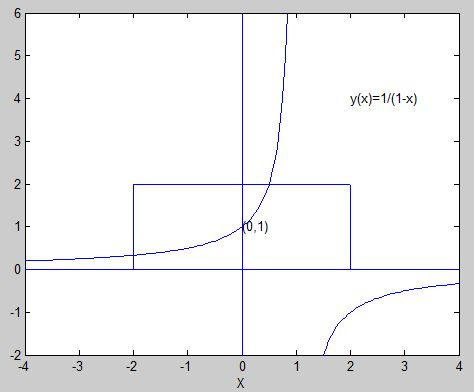
\includegraphics[width=200pt]{1-3-8}\\
图中解曲线在到达区间I的右端点之前离开矩形I
\end{note}
\subsubsection{一阶线性微分方程}
\begin{theorem}
  在两个系数函数P(x)与Q(x)都连续的某一区间上,求解一阶线性微分方程
  \begin{equation}
    \frac{dy}{dx}+P(x)y=Q(x)
    \label{equation 1}
  \end{equation}
  通过对\ref{equation 1}两边乘以适当的积分因子,可以得到一种标准解法,我们乘以
  \begin{equation}
   {\bf  \rho(x)=e^{\int P(x)dx}}
    \label{equation 2}
  \end{equation}
 结果为
 \begin{equation}
    e^{\int P(x)dx} \frac{dy}{dx}+P(x)e^{\int P(x)dx}y=Q(x)e^{\int P(x)dx}
    \label{equation 3}
  \end{equation}
  方程\ref{equation 3}的左边是$y(x)e^{\int P(x)dx}$的微分
  两边积分,最后求出\ref{equation 1}的通解为:
  \begin{equation}
    y(x)=e^{-\int P(x)dx}({\int {Q(x)e^{\int P(x)}dx} }+C)
  \end{equation}
\end{theorem}

\subsubsection{替换方法和恰当方程}
\begin{theorem}
  形如$\frac{dy}{dx}=F(ax+by+c)$ 的微分方程可以通过变换$v=ax+by+c$ 将其变化分离变量型
\end{theorem}
\subsubsection{恰当微分方程}
\begin{theorem}
  {\bf (恰当型判别准则)}假设在矩形开区域$R:a<x<b,c<y<d$ 上,函数M(x,y),N(x,y)连续且有连续一阶偏导数,那么微分方程
  \begin{equation}
  M(x,y)dx+N(x,y)dy=0
\end{equation}
是恰当型的充要条件是
\begin{equation}
  \frac{\partial M}{\partial y}=\frac{\partial N}{\partial x}
  \label{equation 4}
\end{equation}
在矩形R上成立.即存在R上的函数F(x,y), 满足$\frac{\partial f}{\partial x}=M,\frac{\partial f}{\partial y}=N$ 的充要条件是式\ref{equation 4}在矩形R 上成立.
\end{theorem}

\begin{note}
  一般的,为了求解恰当方程$M(x,y)dx+N(x,y)dy=0$, 我们执行以下步骤: \newline
  首先,把M(x,y) 对x 进行积分,且写成下面的形式
  $$
  F(x,y)=\int M(x,y)dx+g(y)
  $$
  然后通过$\frac{\partial F}{\partial y}=N(x,y)$ 求出g(y), 这样就得到方程的隐式解 $F(x,y)=C$
\end{note}
\begin{example}
  求解微分方程$(6xy-y^2)dx+(4y+3x^2-3xy^2)dy=0$ \newline
  解:设$M(x,y)=(6xy-y^2),N(x,y)=(4y+3x^2-3xy^2)$ 因为
  $$
  \frac{\partial M}{\partial y}=6x-3y^2=\frac{\partial N}{\partial x}
  $$
  所以方程是恰当的
  $$
  F(x,y)=\int M(x,y)dx+g(y)=\int (6xy-y^2)dx+g(y)=3x^2y-xy^3+g(y)
  $$
  然后对y进行微分,并设$\frac{\partial f}{\partial y}=N(x,y)$ 得到
  $$
  \frac{\partial f}{\partial y}=3x^2-3xy^2+g'(y)=4y+3x^2-3xy^2
  $$
  整理得到:$g'(y)=4y$, 于是$g(y)=2y^2+C_1$, 从而
  $$
  F(x,y)=3x^2y-xy^3+2y^2+C_1
  $$
  因此微分方程的隐式通解为$$3x^2y-xy^3+2y^2=C$$
\end{example}

\subsection{数值逼近}
\subsubsection{欧拉方法}
已知初值问题
\begin{equation}
  \frac{dy}{dx}=f(x,y),y(x_0)=y_0.
\end{equation}
{\bf 步长为h的欧拉方法}:应用迭代公式
\begin{equation}
  y_{n+1}=y_n+hf(x_n,y_n) ~~~(n\geqslant 0)
\end{equation}
来依次计算在各个点$x_1,x_2,x_3,\ldots,x_n$ 对真实解y=f(x)的真实值$y(x_1),y(x_2),\ldots,y(x_n)$ 的逼近值$y_1,y_2,\ldots,y_n$
\newline

\subsubsection{改进的欧拉方法}
已知初值问题
\begin{equation}
  \frac{dy}{dx}=f(x,y),y(x_0)=y_0.
\end{equation}
假设对步长h执行n步以后,已经得到在$x_n=x_0+nh$ 点解的真值$y(x_n)$ 逼近值$y_n$, 可应用欧拉方法来获得在点$x_{n+1}=x_n+h$ 的解的真值的一个初步估计,即称之为$u_{n+1}$ 而不是$y_{n+1}$ ,则
\begin{equation}
  u_{n+1}=y_n+hf(x_n,y_n)=y_n+hk_1. \quad k_1=f(x_n,y_n)
\end{equation}
既然$u_{n+1}\thickapprox y(x_{n+1})$, 可取$k_2=f(x_{n+1},y_{n+1})$ 作为解曲线$y=f(x)$在$x=x_{x+1}$ 点的斜率的第二个估计. \newline
当然,我们已经求出在$x=x_n$的近似斜率$k_1=f(x_n,y_n)$. 为了获得在整个区间$[x_n,x_{x+1}]$ 上解曲线平均斜率的更加精确的估计,为什么不平均这两个斜率呢? \newline 这个思想就是改进的欧拉方法的本质.
\begin{theorem}
  {\bf 算法~~~改进的欧拉方法} \newline
给定初值问题
\begin{equation}
  \frac{dy}{dx}=f(x,y),y(x_0)=y_0.
\end{equation}
步长为h的欧拉方法:应用迭代公式
$
\begin{cases}
  k_1=f(x_n,y_n) \\
  u_{n+1}=y_n+hk_1 \\
  k_2=f(x_{n+1},y_{n+1}) \\
  y_{n+1}=y_n+\frac{1}{2}h(k_1+k_2)
\end{cases}
$
\\
来依次计算$y=f(x)$在点$x_1,x_2,x_3,\ldots,x_n$的真值$y(x_1),y(x_2),\ldots,y(x_n)$ 的逼近值$y_1,y_2,\ldots,y_n$. 
\end{theorem}
\begin{note}
  改进后的欧拉方法使用的是一种称为{\bf 预测-校正}方法的一类数值技术之一. 首先计算下一个y值的预测值$u_{n+1}$ ,然后它自我校正. 这样步长为h的改进的欧拉方法\\
  由使用预测值
  \begin{equation}
    u_{n+1}=y_n+hf(x_n,y_n)
  \end{equation}
  和校正值
  \begin{equation}
    y_{n+1}=y_n+\frac{1}{2}h(f(x_n,y_n)+f(x_{n+1},y_{n+1}))
  \end{equation}
  构成.
\end{note}

\subsubsection{龙格-库塔方法}

\textbf{COERVIT\'E}
Une fonction f d\'efinie sur un espace norm\'e X \`a valeurs dans $ \bar{\R}:=\R\cup\{-\infty,+\infty\}$ est dite coercive sur une partie non born\'ee $ P$ de $X$ si
$$ \lim_{\mytop{\| x\| \to +\infty}{x\in P}}f(x)=+\infty $$

ou de mani\`ere plus pr\'ecise
$$
\forall\,\nu\in\R,\quad \exists\,\rho\geqslant0:\quad (x\in X ~\mbox{et}~ \|x\|\geqslant\rho) \quad\Longrightarrow\quad f(x)\geqslant\nu.
$$

Il revient au m\^eme de dire que les intersections avec P des ensembles de sous-niveau de la fonction sont born\'ees :
$$
\forall\,\nu\in\R,\qquad\{x\in P: f(x)\leqslant\nu\}~\mbox{est born\'e.}
$$
Si l'on ne sp\'ecifie pas la partie P, il est sous-entendu que P=X.

\underline{Cas d'une forme bilin\'eaire} \newline
Plus sp\'ecifiquement, une forme bilin\'eaire $a:X\times X\to\R$ est dite coercive si elle v\'erifie :
$$
\exists\,\alpha>0,\quad\forall\,x\in X:\qquad a(x,x) \geqslant \alpha\|x\|^2.
$$
Certains auteurs pr\'ef\`erent utiliser l'appellation X-elliptique pour cette derni\`ere d\'efinition. Celle-ci intervient entre autres dans le th\'eor\`eme de Lax-Milgram et la th\'eorie des op\'erateurs elliptiques, accessoirement dans la m\'ethode des \'el\'ements finis.

\underline{Lien entre les d\'efinitions}\newline
Dans le cas où a est une forme bilin\'eaire, en posant $f(u)=a(u,u)$ on a \'equivalence entre la coercivit\'e de a et celle de $f$. En effet, $\scriptstyle\lim_{\| x\|\to\infty}f(x)=+\infty $implique qu'il existe $R>0 $tel que $\scriptstyle\|x\|\geqslant R\Rightarrow f(x)\geqslant 1$. Ainsi:
$$
\left(\frac{R}{\|u\|}\right)^2a(u,u)=a\left(\frac{R}{\|u\|}u,\frac{R}{\|u\|}u\right)=f\left(\frac{R}{\|u\|}u\right)\geqslant 1
$$
et
$$
a(u,u)\geqslant\left(\frac{\|u\|}{R}\right)^2.
$$
维基百科上没有直接给出coercivit\'e的定义, 但是按照维基百科的解释, 我觉得coercivit\'e的定义是
$$
 \alpha=\left(\frac{1}{R}\right)^2
$$

\bigskip
\textbf{Application contractante}\newline
Une application contractante, ou contraction, est une application k-lipschitzienne avec $0 \geq k \le 1$
\bigskip

\textbf{Th\'eor\`eme du point fixe pour une application contractante}\newline
Soient $ E$  un espace m\'etrique complet (non vide) et $ f$  une application $ k$ -contractante de $ E$  dans $ E$ . Il existe un point fixe unique $x^*$ de f (c'est-\`a-dire un $x^*$ dans $ E$  tel que $ f(x^* ) = x^*)$ . De plus, toute suite d'\'el\'ements de E v\'erifiant la r\'ecurrence
$$x_{n+1}=f(x_n)$$
v\'erifie la majoration
$$d(x_n,x^*) \le \frac {k^n}{1-k} d(x_0,x_1)$$
donc converge vers $x^*$
\bigskip

\textbf{In\'egalit\'e de Poincar\'e}
un r\'esultat de la th\'eorie des espaces de Sobolev\\
Cette in\'egalit\'e permet de borner une fonction \`a partir d'une estimation sur ses d\'eriv\'ees et de la g\'eom\'etrie de son domaine de d\'efinition\\
L'in\'egalit\'e de Poincar\'e classique
Soit $p$, tel que $ 1 \leq p < \infinity$  et $\Omega$ un ouvert de largeur finie (born\'e dans une direction). Alors il existe une constante  $  C$  , d\'ependant uniquement de $\Omega$ et $p$, telle que, pour toute fonction $u$   de l'espace de Sobolev $W_0^{1,p(\Omega)}$
$$
\| u \|_{L^{p} (\Omega)} \leq C \| \nabla u \|_{L^{p} (\Omega)}
$$

\section{Formula}
\subsection{Tylor series}
$$
e^x
= 1+x+\frac{ x^2}{2!}
+ \ldots +
\frac{ x^n}{n!}
+0(x^n)
=\sum_{k=0}^{+\infty}\frac{ x^k}{k!}
\quad x \in \R
$$

$$
\sin x=x-\frac{ x^3}{3!}+\frac{ x^5}{5!}+\ldots+ (-1)^n \frac{x^{2n+1}}{(2n+2)!}+
0(x^{2n+1})
=
\sum_{n=0}^{+\infty} \frac{(-1)^n}{(2n+1)!} x^{2n+1}
\quad x \in \R
$$

$$
\cos x =
1 - \frac{ x^2}{2!} + \frac{ x^4}{4!}
+ \ldots +
(-1)^n \frac{ x^{2n}}{(2n)!} + 0(x^{2n+1})
\sum_{n=0}^{+\infty} \frac{(-1)^n}{(2n)!} x^{2n}
\quad x \in \R
$$

$$
\sinh x=x + \frac{ x^3}{3!}+\frac{ x^5}{5!}+\ldots+ \frac{x^{2n+1}}{(2n+1)!}+
0(x^{2n+2})
=
\sum_{n=0}^{+\infty} \frac{x^{2n+1}}{(2n+1)!}
\quad x \in \R
$$

$$
\cosh x =
1 + \frac{ x^2}{2!} + \frac{ x^4}{4!}
+ \ldots +
\frac{ x^{2n}}{(2n)!} + 0(x^{2n+1})
$$

$$
(1+x)^\alpha = 1+\frac{ \alpha}{1!}x + \frac{ \alpha(\alpha-1)}{2!}x^2
+\ldots+
\frac{ \alpha(\alpha-1)\ldots(\alpha-n+1)}{n!}x^n+
0(x^n)
$$

$$
\frac{ 1}{1+x}= 1 -x +x^2-x^3+\ldots +(-1)^n x^n +0(x^n)=\sum_{k=0}^{+\infty}(-1)^kx^k
$$

$$
\frac{ 1}{1-x}= 1 +x +x^2-x^3+\ldots +x^n +0(x^n)=\sum_{k=0}^{+\infty}x^k
$$

$$
\sqrt{1+x}= 1+\frac{ x}{2}-\frac{ 1}{2\cdot 4}x^2+ \frac{ 1\cdot3}{2\cdot4\cdot6}x^3
+\ldots+
(-1)^{n-1} \frac{1\cdot3\ldots(2n-3)}{2\cdot4\ldots(2n)}x^n +0(x^n)
$$

$$
\sqrt{1-x}= 1-\frac{ x}{2}-\frac{ 1}{2\cdot 4}x^2- \frac{ 1\cdot3}{2\cdot4\cdot6}x^3
-\ldots-
(-1)^{n-1} \frac{1\cdot3\ldots(2n-3)}{2\cdot4\ldots(2n)}x^n -0(x^n)
$$

$$
\frac{ 1}{\sqrt{1+x}}
= 1-\frac{ x}{2}+\frac{ 1\cdot3}{2\cdot 4}x^2
+\ldots+
(-1)^{n-1} \frac{1\cdot3\ldots(2n-1)}{2\cdot4\ldots(2n)}x^n +0(x^n)
$$

$$
\frac{ 1}{\sqrt{1-x}}
= 1+\frac{ x}{2}+\frac{ 1\cdot3}{2\cdot 4}x^2
+\ldots+
\frac{1\cdot3\ldots(2n-1)}{2\cdot4\ldots(2n)}x^n +0(x^n)
$$

$$
\log (1+x)=
x-\frac{ x^2}{2}+\frac{ x^3}{3}+\ldots+ (-1)^{n-1} \frac{ x^n}{n}+0(x^n)
=\sum_{k=1}^{+\infty}\frac{(-1)^{n-1}x^n}{n}
\quad x\in(-1,1]
$$

$$
\arctan x=x-\frac{ x^3}{3}+\frac{ x^5}{5}+\ldots+ (-1)^n \frac{x^{2n+1}}{2n+1}+
0(x^{2n+2})
=
\sum_{n=0}^{+\infty} \frac{(-1)^n}{2n+1} x^{2n+1}
\quad x\in[-1,1]
$$

$$
\arcth x=x+\frac{ x^3}{3}+\frac{ x^5}{5}+\ldots+ \frac{x^{2n+1}}{2n+1}+
0(x^{2n+2})
=
\sum_{n=0}^{+\infty} \frac{1}{2n+1} x^{2n+1}
\quad x\in[-1,1]
$$

\red{arcsin arcsh tan待验证}

$$
\arcsin x=
x+ \frac{ 1}{2\cdot3}x^3+\frac{1\cdot3}{2\cdot4\cdot5}x^5
+\ldots+
\frac{ 1\cdot3\cdot(2n-1)}{2\cdot4\cdot(2n)\cdot(2n+1)}x^{2n+1}+0(x^{2n+2})
$$

$$
\arcsh x=
x-\frac{ 1}{2\cdot3}x^3+\frac{1\cdot3}{2\cdot4\cdot5}x^5
+\ldots+
\frac{ (-1)^n \cdot1\cdot3\cdot(2n-1)}{2\cdot4\cdot(2n)\cdot(2n+1)}x^{2n+1}+0(x^{2n+2})
$$

$$
\tan x=
x+\frac{ x^3}{3}+\frac{2}{15}x^5+\frac{ 11}{315}x^7+0(x^8)
$$


\subsection{常用的初等数学公式}
\subsubsection{有限项数项级数}
$$
1^2 + 2^2 +3^2+\ldots+n^2=\frac{ n(n+1)(n+2)}{6}
$$

$$
1^3 + 2^3 +3^3+\ldots+n^3=\frac{ n^2(n+1)^2}{4}
$$

$$
1^2+3^2+5^2+\ldots+(2n-1)^2=\frac{n(4n^2-1)}{3}
$$

$$
1^3 + 3^3 +5^3+\ldots+(2n-1)^3=n^2(2n^2-1)
$$

\subsubsection{双曲函数}
$$
\sh x=\frac{e^x - e^{-x}}{2}, \quad \ch x=\frac{e^x+e^{-x}}{2}, \quad \dth x = \frac{ \sh x}{\ch x}=\frac{e^x-e^{-x}}{e^x + e^{-x}}
$$

\subsubsection{三角}
$$
\sin ^2 \alpha + \cos^2 \alpha=1
$$

$$
\frac{ \sin x}{\cos x}=\tan x, \quad
\frac{ \cos x}{\sin x}=\cot x, \quad
\csc x=\frac{1}{\sin x}, \quad
\sec x=\frac{ 1}{\cos x}, \quad
1+\tan^2 x=\sec^2 x,\quad
1+\cot^2 x=\csc^2 x
$$

万能公式
$$
\tan \frac{x}{2}=t \Rightarrow
\cos x =\frac{ 1-t^2}{1+t^2},\quad
\sin x=\frac{2t}{1+t^2},\quad
dx=\frac{2}{1+t^2}dx
$$

和差公式
$$
\sin(x\pm y)=\sin x \cos y \pm \cos x \sin y,\quad \cos(x \pm y)=\cos x \cos y \mp \sin x \sin y
$$

$$
\tan(x \pm y)=\frac{\tan x \pm \tan y}{1 \mp \tan x \tan y}, \quad
\cot (x\pm y)=\frac{\cot x \cot y \mp 1}{\cot y \pm \cot x}
$$

$$
\sin x+\sin y=2\sin \frac{x+y}{2} \cos \frac{ x -y }{2}, \quad
\sin x-\sin y=2\cos \frac{x+y}{2} \sin \frac{ x -y }{2}
$$

$$
\cos x+\cos y=2\cos \frac{x+y}{2} \cos \frac{ x -y }{2}, \quad
\cos x-\cos y=2\sin \frac{x+y}{2} \sin \frac{ x -y }{2}
$$

$$
\cos x \cos y=\frac{ 1}{2}[\cos(x-y)+\cos(x+y)]
$$

$$
\sin x \sin y=\frac{ 1}{2}[\cos(x-y)-\cos(x+y)]
$$

$$
\sin x \cos y=\frac{ 1}{2}[\sin(x-y)+\sin(x+y)]
$$

被角公式
$$
\sin 2x=2\sin x \cos x,\quad \cos 2x=\cos^2 x-\sin ^2 x=1-2\sin^2 x=2\cos^2 x -1
$$

任意三角形的基本关系
$$
\frac{a}{\sin A}=
\frac{b}{\sin B}=
\frac{c}{\sin C}=
2R(\mbox{正弦定理})
$$

$$
a^2=b^2+c^2-2bc\cos A (\mbox{余弦定理})
$$

$$
S= \frac{ 1}{2}ab\sin C=\sqrt{p(p-a)(p-b)(p-c)}~\mbox{where}~p=\frac{1}{2}(a+b+c)~ (\mbox{面积公式})
$$

\subsubsection{初等几何}
\textbf{扇形:}
弧长$l=\alpha \cdot R$, \quad
面积$S=\dfrac{1}{2}l\cdot R=\dfrac{1}{2}\alpha R^2$

\textbf{正圆锥}
体积$V=\dfrac{1}{3}\pi r^3 h$ , \quad
侧面积$S=\pi rl$, \quad
全面积$A=\pi r(r+l)$

\textbf{截圆锥}
体积$V=\dfrac{\pi h}{3}(R^2+r^2+Rr)$, \quad
侧面积$S=\pi l(R+r)$

\subsubsection{中值定理}
拉格朗日中值定理: $f(b)-f(a)=f'(\xi)(b-a)$

柯西中值定理: $$\frac{f(b)-f(a)}{g(b)-g(a)}=\frac{f'(\xi) }{g'(\xi)}$$
\subsubsection{曲率}
弧微分公式: $ds=\sqrt{1+y'^2}dx$,其中$y'=\tan \alpha$

平均曲率: $K=|\frac{\Delta\alpha}{\Delta s}|$ 其中$\Delta \alpha$:从$M$点到$M'$点,切线斜率的倾角变化量; $\Delta s$:$MM'$弧长

M点的曲率: $K=lim_{\Delta s \to 0}|\frac{\Delta\alpha}{\Delta s}|=|\frac{d \alpha}{ds}|=\frac{|y''|}{\sqrt{(1+y'^2)^3}}$

直线: $K=0$

半径为$a$的圆: $K=\frac{1}{a}$

\subsection{积分表}
\textbf{导数公式}
$$
(\tan x)'=\sec ^2 x,\quad
(\cot x)'=-\csc^2 x,\quad
(a^x)'=a^x\ln a,\quad
(\log_a x)'=\frac{1}{x \ln a}
$$

$$
(\arcsin x)'=\frac{1}{\sqrt{1-x^2}}, \quad
(\arccos x)'=-\frac{1}{\sqrt{1-x^2}}, \quad
(\arctan x)'=\frac{1}{1+x^2}, \quad
(\arccot x)'=-\frac{1}{1+x^2}
$$

$$
d(\frac{1}{|x|})=-\frac{1}{x|x|}dx, \quad |x|=sgn(x)\cdot x
$$

\textbf{含有$ax+b$的积分}

$$
\int \frac{dx}{ax+b}=\frac{1}{a}\ln|ax+b|+C
$$

$$
\int \frac{dx}{x(ax+b)}=-\frac{1}{b}\ln|\frac{ax+b}{x}|+C
$$

$$
\int \frac{dx}{x^2(ax+b)}=-\frac{ 1}{bx}+\frac{ a}{b^2}\ln |\frac{ax+b}{x}|+C
$$

\textbf{含有$\sqrt{ax+b}$的积分}
$$
\int \sqrt{ax+b}dx=\frac{2}{3a}\sqrt{(ax+b)^3}+C
$$

$$
\int x\sqrt{ax+b}dx=\frac{2}{15a^2}(3ax-2b)\sqrt{(ax+b)^3}+C
$$

$$
\int \frac{x}{\sqrt{ax+b}}dx=\frac{2}{3a^2}(ax-2b)\sqrt{ax+b}+C
$$

\textbf{含有$x^2 \pm a^2$的积分}
$$
\int \frac{dx}{x^2+a^2}=\frac{1}{a}\arctan \frac{x}{a}+C
$$
$$
\int \frac{dx}{x^2-a^2}=\frac{1}{2a}\ln |\frac{x-a}{x+a}|+C
$$
\textbf{含有$ax^2+b(a>0)$的积分}
$$
\int \frac{dx}{ax^2+b}=
\left\{
		\begin{array}{ll}
			\frac{1}{\sqrt{ab}}\arctan \sqrt{\frac{a}{b}}x+C & (b>0) \\
			\frac{1}{2\sqrt{-ab}}\ln|\frac{\sqrt{a}x-\sqrt{-b}}{\sqrt{a}x+\sqrt{-b}}+C & (b<0)
		\end{array}
		\right.
$$

$$
\int \frac{x}{ax^2+b}dx=\frac{1}{2a}\ln |ax^2+b|+C
$$

$$
\int \frac{dx}{x(ax^2+b)}=\frac{1}{2b}\ln \frac{x^2}{|ax^2+b|}+C
$$

\textbf{含有$ax^2+bx+c(a>0)$的积分}
$$
\int \frac{ dx}{ax^2+bx+c}=
\left\{
		\begin{array}{ll}
		 \frac{2}{\sqrt{4ac-b^2}}\arctan \frac{2ax+b}{\sqrt{4ac-b^2}}+C & (b^2<4ac) \\
		 \frac{1}{\sqrt{b^2-4ac}}\ln|\frac{2ax+b-\sqrt{b^2-4ac}}{2ax+b+\sqrt{b^2-4ac}}|+C & (b^2>4ac)
		\end{array}
		\right.
$$

$$
\int \frac{x}{ax^2+bx+c}dx=\frac{1}{2a}\ln|ax^2+bx+c|-\frac{b}{2a}\int \frac{dx}{ax^2+bx+c}
$$

\textbf{含有$\sqrt{x^2+a^2}(a>0)$的积分}
$$
\int \frac{dx}{\sqrt{x^2+a^2}}=\arcsh \frac{x}{a}+C_1=\ln(x+\sqrt{x^2+a^2})+C,\quad \big( \ln(x+\sqrt{1+x^2})\big)'=\frac{1}{\sqrt{1+x^2}}
$$

$$
\int \sqrt{x^2+a^2}dx=\frac{x}{2}\sqrt{x^2+a^2}+\frac{a^2}{2}\ln(x+\sqrt{x^2+a^2})+C
$$

\textbf{含有$\sqrt{x^2-a^2}(a<0)$的积分}
$$
\int \frac{dx}{\sqrt{x^2-a^2}}=\frac{x}{|x|}\arch \frac{|x|}{a}+C_1=
\ln|x+\sqrt{x^2-a^2}|+C
$$

$$
\int \frac{x}{\sqrt{x^2-a^2}}dx=\sqrt{x^2-a^2}+C
$$

$$
\int \frac{dx}{x\sqrt{x^2-a^2}}=\frac{1}{a}\arccos \frac{a}{|x|}+C
$$

\textbf{含有$\sqrt{a^2-x^2}(a>0)$的积分}
$$
\int \frac{dx}{\sqrt{a^2-x^2}}=\arcsin \frac{x}{a}+C
$$

$$
\int \frac{x}{\sqrt{a^2-x^2}}dx=-\sqrt{a^2 - x^2}+C
$$

$$
\int \frac{dx}{x\sqrt{a^2-x^2}}=\frac{1}{a}\ln \frac{a-\sqrt{a^2 - x^2}}{|x|}+C
$$

\textbf{含有$\sqrt{\pm ax^2+bx+c}(a>0)$的积分}
$$
\int \frac{dx}{\sqrt{ax^2+bx+c}}=\frac{1}{\sqrt{a}}
\ln|2ax+b+2\sqrt{a}\sqrt{ax^2+bx+c}+C|
$$
$$
\int \sqrt{ax^2+bx+c}dx=\frac{2ax+b}{4a}\sqrt{ax^2+bx+c}+
\frac{4ac-b^2}{8\sqrt{a^3}}
\ln|2ax+b+2\sqrt{a}\sqrt{ax^2+bx+c}+C|
$$
\textbf{含有$\sqrt{\pm \frac{x-a}{x-b}}$或$\sqrt{(x-a)(x-b)}$的积分}
$$
\int \sqrt{\frac{x-a}{x-b}}dx=(x-b)\sqrt{\frac{x-a}{x-b}}+
(b-a)\ln (\sqrt{|x-a|}+\sqrt{|x-b|})+C
$$

$$
\int \sqrt{\frac{x-a}{b-x}}dx=(x-b)\sqrt{\frac{x-a}{b-x}}+
(b-a)\arcsin \sqrt{\frac{x-a}{b-a}}+C
$$

$$
\int \frac{dx}{\sqrt{(x-a)(b-x)}}=2\arcsin \sqrt{\frac{x-a}{b-a}}+C \quad(a<b)
$$

$$
\int \sqrt{(x-a)(b-x)}=\frac{2x-a-b}{4}\sqrt{(x-a)(b-x)}
+ \frac{(b-a)^2}{4}\arcsin \sqrt{\frac{x-a}{b-a}}+C \quad(a<b)
$$
\textbf{含有三角函数的积分}
$$
\int \sin xdx=-\cos x +C
$$

$$
\int \cos xdx =\sin x +C
$$

$$
\int \tan xdx=-\ln|\cos x|+C
$$

$$
\int \cot xdx=\ln|\sin x|+C
$$

$$
\int \sec xdx=\ln|\tan(\frac{\pi}{4}+\frac{x}{2})|+C=\ln|\sec x+ \tan x|+C
$$

$$
\int \csc xdx=\ln|\tan \frac{x}{2}|=\ln|\csc x-\cot x|+C
$$


$$
\int \sin^n x dx=-\frac{1}{n}\sin^{n-1}x \cos x + \frac{n-1}{n}\int \sin^{n-2}x dx
$$
$$
\int \cos^n x dx=\frac{1}{n}\cos^{n-1}x \sin x + \frac{n-1}{n}\int \cos^{n-2}x dx
$$


$$
\int \frac{dx}{a+b\sin x}=\frac{2}{\sqrt{a^2-b^2}}\arctan \frac{a \tan \frac{x}{2}+b}{\sqrt{a^2-b^2}}+C \quad(a^2>b^2)
$$

$$
\int \frac{dx}{a+b\cos x}=\frac{2}{a+b} \sqrt{\frac{a+b}{a-b}}\arctan(\sqrt{\frac{a-b}{a+b}}\tan \frac{x}{2})+C \quad (a^2>b^2)
$$


$$
\int \frac{ dx}{a^2 \cos^2 x+b^2\sin^2 x}=\frac{ 1}{ab} \arctan(\frac{b}{a}\tan x)+C, \quad
\frac{\frac{1}{\cos^2}dx}{a^2+b^2\tan^2 x}=\frac{d \tan x}{a^2 + b^2 \tan^2 x}
$$

\textbf{含有反三角函数的积分(其中($a>0$))}
$$
\int \arcsin \frac{x}{a}dx=x\arcsin \frac{x}{a}+\sqrt{a^2-x^2}+C
$$

$$
\int x\arcsin \frac{x}{a}dx=(\frac{x^2}{2}-\frac{ a^2}{4})\arcsin \frac{x}{a}+ \frac{x}{4}\sqrt{a^2-x^2}+C
$$

$$
\int \arccos \frac{x}{a}dx=x \arccos \frac{x}{a}-\sqrt{a^2-x^2}+C
$$

$$
\int x\arccos \frac{x}{a}dx=(\frac{x^2}{2}-\frac{ a^2}{4})\arccos \frac{x}{a}- \frac{x}{4}\sqrt{a^2-x^2}+C
$$

$$
\int \arctan \frac{x}{a}dx=x \arctan \frac{x}{a}-\frac{a}{2}\ln(a^2+x^2)+C
$$

$$
\int x \arctan \frac{x}{a}dx=\frac{1}{2}(a^2+x^2)\arctan \frac{x}{a}- \frac{a}{2}x+C
$$
\textbf{含有指数函数的积分}
$$
\int a^xdx=\frac{1}{\ln a}a^x+C
$$
$$
\int e^{ax}dx=\frac{ 1}{a}e^{ax}+C
$$

\textbf{含有对数函数的积分}
$$
\int \ln xdx=x\ln x-x +C
$$

$$
\int (\ln x)^n dx=x(\ln x)^n -n \int (\ln x)^{n-1}dx
$$
\textbf{含有双曲函数的积分}
$$
\int \sh xdx=\ch x+C
$$

$$
\int \ch xdx=\sh x+C
$$

$$
\int \dth xdx=\ln \ch x+C
$$
\textbf{定积分}
$$
\int_{-\pi}^{\pi} \cos nx dx=
\int_{-\pi}^{\pi} \sin nx dx=0
$$
$$
\int_{-\pi}^{\pi} \cos mx\sin nx dx=0
$$

$$
\int_{-\pi}^{\pi} \cos mx\cos nx dx=
\left\{
		\begin{array}{ll}
		 0 & m \neq n \\
		 \pi & m = n
		\end{array}
		\right.
$$

$$
\int_{-\pi}^{\pi} \sin mx\sin nx dx=
\left\{
		\begin{array}{ll}
		 0 & m \neq n \\
		 \pi & m = n
		\end{array}
		\right.
$$

$$
\int_{0}^{\pi} \sin mx\sin nx dx=
\int_{0}^{\pi} \cos mx\cos nx dx=
\left\{
		\begin{array}{ll}
		 0 & m \neq n \\
		 \pi & m = n
		\end{array}
		\right.
$$

$$
I_n=\int_{0}^{\pi/2} \sin^n xdx=\int_{0}^{\pi/2}\cos^n xdx=\frac{n-1}{n}I_{n-2},\quad
I_1=1, I_0=\frac{ \pi}{2}
$$

\subsection{Transformations}
\subsubsection{Dirac}
Soit
\begin{equation}
		 \delta _{\varepsilon}(t)=
\left\{
		\begin{array}{ll}
		0 & t<0 \\
		\frac{ 1}{\varepsilon} & 0\leq t \leq \varepsilon \\
		0 & t> \varepsilon
		\end{array}
		\right.
\end{equation}
\begin{definition}
\begin{equation}
\delta (t)=\lim_{\varepsilon \to 0}\delta _{\varepsilon}(t)=
\left\{
		\begin{array}{ll}
		 0 & t\neq 0 \\
		 \infty & t=0
		\end{array}
		\right.
\end{equation}
$$
\int_{-\infty}^{+\infty}\delta (t)dt
=\lim_{\varepsilon \to 0}\int_{-\infty}^{+\infty} \delta_{\varepsilon}(t)dt
=\lim_{\varepsilon \to 0}\int_{0}^{\varepsilon}\frac{1}{\varepsilon}dt
=1
$$
\end{definition}
Propri\'et\'es:

\subsubsection{Transformation de Fourrier}
\textbf{Serie de Fourrier}
给定一个周期为T的函数x(t),那么它可以表示为无穷级数:
\begin{equation}
		x(t)=\sum _{k=-\infty}^{+\infty}a_k\cdot e^{ik(\frac{2\pi}{T})t}\eqspace (i\text{为虚数单位})
\label{serie.fourrier.fonction}
\end{equation}
其中,$a_k$可以按下式计算:
$$
a_k=\frac{1}{T}\int_{T}x(t)\cdot e^{-ik(\frac{2\pi}{T})t}dt
$$
注意到$f_k(t)=e^{ik(\frac{2\pi}{T})t}$是周期为T的函数,故k 取不同值时的周期信号具有谐波关系(即它们都具有一个共同周期T).\newline
$k=0$时,\eqref{serie.fourrier.fonction} 式中对应的这一项称为直流分量,也就是x(t)在整个周期的平均值.\newline
$k=\pm 1$时具有基波频率$\omega_0=\frac{2\pi}{T}$,称为一次谐波或基波,类似的有二次谐波,三次谐波等等。

\textbf{三角函数族的正交性}
所谓的两个不同向量正交是指它们的内积为0,这也就意味着这两个向量之间没有任何相关性,例如,在三维欧氏空间中,互相垂直的向量之间是正交的。事实上,正交是垂直在数学上的一种抽象化和一般化。一组n个互相正交的向量必然是线性无关的,所以必然可以张成一个n维空间,也就是说,空间中的任何一个向量可以用它们来线性表出。三角函数族的正交性用公式表示出来就是:
$$\int _{0}^{2\pi}\sin (nx)\cos (mx) \,dx=0;$$
$$\int _{0}^{2\pi}\sin (nx)\sin (mx) \,dx=0;(m\ne n)$$
$$\int _{0}^{2\pi}\cos (nx)\cos (mx) \,dx=0;(m\ne n)$$
$$\int _{0}^{2\pi}\sin (nx)\sin (nx) \,dx=\pi;$$
$$\int _{0}^{2\pi}\cos (nx)\cos (nx) \,dx=\pi;$$
\bigskip

$$F(w)=\int_{-\infty}^{+\infty}f(t)e^{-iwt}dt$$
称为$f(t)$的Fourrier变换,记为$F[f(t)]$
$$\frac{ 1}{2\pi}\int_{-\infty}^{\infty}F(w)e^{iwt}dw$$称为$F(w)$的Fourrier逆变换,记为$F^{-1}[F(w)]$
$$f(t) \longleftrightarrow F(w)$$一一对应,称为一组Fourrier变换对,其中$f(t)$称为原像函数,$F(w)$称为像函数.
\begin{example}
\begin{equation}
f(t)=
\left\{
		\begin{array}{ll}
			1 & |t| \leq 1 \\
			0 & |t| > 1
		\end{array}
		\right.
\end{equation}
\begin{eqnarray}
 F(w)=\int_{-\infty}^{+\infty} f(t)e^{-iwt}dt=\int_{-1}^{+1}e^{-iwt}=\frac{2\sin w}{w}
\end{eqnarray}
%% \includegraphics[width=\textwidth]{sinx_x}
\end{example}

\begin{example}
\begin{equation}
f(t)=
\left\{
		\begin{array}{ll}
			0 & t \leq 1 \\
			0 & |t| > 1
		\end{array}
		\right.
\end{equation}
\begin{eqnarray}
 F(w)=\int_{-\infty}^{+\infty} f(t)e^{-iwt}dt=\int_{-1}^{+1}e^{-iwt}=\frac{2\sin w}{w}
\end{eqnarray}
\end{example}

\subsection{算子(laplace, gradien etc.)}
\textbf{拉普拉斯算子: 梯度的散度}
$$\laplace f = \mbox{div} (\vec{\mbox{grad}}f)$$

Cart\'esien: $$\laplace f = \sum_{i=1}^n \frac{\partial^2 f }{\partial x_i^2} $$

函数的拉普拉斯算子也是该函数的黑塞矩阵的迹 $\laplace f = tr(H(f))$

极坐标下的拉普拉斯算子表示法
$$\laplace f = \frac{ 1}{\rho}\frac{\partial  }{\partial \rho}(\rho \frac{\partial  f}{\partial \rho}) + \frac{ 1}{\rho^2}\frac{\partial ^2 f}{\partial\theta^2} + \frac{\partial^2 f}{\partial z^2}$$

\bigskip
\textbf{Equation de poisson}
$$\laplace \varphi = f$$
si $f=0$, 那么泊松方程就会变成一个齐次方程, 称为拉普拉斯方程

\bigskip
\textbf{高斯}

高斯公式用散度表示为:
$$
\iiint_{\Omega}\mathrm{div}\mathbf{A}dv=
\int\!\!\!\!\int_{\Sigma}\!\!\!\!\!\!\!\!\!\!\!\!\!\!\;\;\;\bigcirc\,\,A_{n}dS
=
\int\!\!\!\!\int_{\Sigma}\!\!\!\!\!\!\!\!\!\!\!\!\!\!\;\;\;\bigcirc\,\,\mathbf{A}\cdot d\mathbf{S}
$$
其中Σ是空间闭区域Ω的边界曲面,而
$$
A_n=\mathbf{A}\cdot\mathbf{n}=P\cos\alpha+Q\cos\beta+R\cos\gamma
$$
$$
d\mathbf{S}=\mathbf{n}\cdot S
$$
$n$是向量$A$在曲面$\Sigma$的外侧法向量上的投影。

\bigskip
%\vskip 0.5cm
\textbf{斯托克斯公式}

$\mathbf{R}^3$上的斯托克斯公式
设$S$是分片光滑的有向曲面,$S$的边界为有向闭曲线$Γ$,即$\Gamma=\partial S$,且$Γ$的正向与$S$的侧符合右手规则: 函数$P(x,y,z),Q(x,y,z),R(x,y,z)$都是定义在"曲面$S$连同其边界$Γ$"上且都具有一阶连续偏导数的函数,则有
$$\iint\limits_{S}(\frac{\partial R}{\partial y}-\frac{\partial Q}{\partial z})dydz+(\frac{\partial P}{\partial z}-\frac{\partial R}{\partial x})dzdx+(\frac{\partial Q}{\partial x}-\frac{\partial P}{\partial y})dxdy
=\oint\limits_{\Gamma}Pdx+Qdy+Rdz$$

这个公式叫做$\mathbf{R}^3$上的斯托克斯公式或开尔文-斯托克斯定理、旋度定理。这和函数的旋度有关,用梯度算符可写成
$$
 \int_{S} \nabla \times \mathbf{F} \cdot d\mathbf{S} = \oint_{\partial S} \mathbf{F} \cdot d \mathbf{r}
$$

通过以下公式可以在"对坐标的"曲线积分""和对面积的"面积积分""之间相互转换:
$$
\iint\limits_{\Sigma}\begin{vmatrix} \cos \alpha & \cos \beta & \cos \gamma \\ \frac{\partial}{\partial x} & \frac{\partial}{\partial y} & \frac{\partial}{\partial z} \\ P & Q & R \end{vmatrix}dS=\oint\limits_{\Gamma}Pdx+Qdy+Rdz
$$

\bigskip
\textbf{格林公式}
设闭区域$D$由分段光滑的曲线$\partial D$($\partial D$是$D$取正向的边界曲线)围成,函数$P(x,y)$及$Q(x,y)$在$D$上具有一阶连续偏导数,则有
$$\oint_{\partial D} (Pdx+Qdy) = \iint_D (\frac{\partial Q}{\partial x} - \frac{\partial  P}{\partial y}dxdy)$$

\bigskip
\textbf{格林第一公式}
设函数$u(x,y,z)$和$v(x,y,z)$在闭区域$\Omega$上具有一阶及二阶连续偏导数,则有
$$\iiint_{\Omega} u\laplace v dxdydz
=
\oint\!\oint_{\Sigma} u \frac{\partial v}{\partial n}dS -
\iiint_{\Omega}(
\frac{\partial  u}{\partial x}\frac{\partial v}{\partial x}+
\frac{\partial  u}{\partial y}\frac{\partial v}{\partial y}+
\frac{\partial  u}{\partial z}\frac{\partial v}{\partial z}+
)dxdydz$$
其中$\Sigma$是闭区域$\Omega$的整个边界曲面,$\frac{\partial v}{\partial n}$为函数$v(x,y,z)$沿$\Sigma$的外法线方向的方向导数

更加简洁的写法:
$$
\int_{\Omega}u \laplace v d\Omega = \int_{\Sigma}u \frac{\partial v}{\partial n}d\Sigma - \int_{\Omega} \vec{\mbox{grad}}u \cdot \vec{\mbox{grad}} v d\Omega
$$
也可以用int\'egration par partie 来理解:
div是二次微分, grad是一次微分, div可以看成是在grad的基础上再来一次微分, 而
$ \frac{\partial  v}{\partial n} = <\vec{\mbox{grad}} v,\vec{n}>$, 所以
$\frac{\partial  v}{\partial n}$ 可以理解成一次微分

\bigskip
\textbf{格林第二公式}
设$u(x,y,z)$、$v(x,y,z)$是两个定义在闭区域$\Omega$上的具有二阶连续偏导数的函数,$\frac{\partial u}{\partial n},\frac{\partial v}{\partial n}$依次表示$u(x,y,z)$、$v(x,y,z)$沿$\Sigma$的外法线方向的方向导数,则有
$$\iiint\limits_{\Omega}(u\Delta v - v\Delta u)dxdydz=\oint\!\oint_{\Sigma}(u \frac{\partial v}{\partial n}-v\frac{\partial u}{\partial n})dS$$

\subsection{Other}
负数的对数
$$e^{i\theta}=cos\theta+isin\theta$$
当$\theta=\pi$时,得到:$e^{i\pi}=-1\Rightarrow ln(-1)=i\pi$。
这样,我们可以计算任意负数的自然对数,例如:
$$ln(-5)=ln[(-1)*5]=ln(-1)+ln5=i\pi+ln5$$
(注,这里没有考虑$2k\pi$的周期)

Une matrice
$$
P=
\left(
             \begin{array}{ccc}
               x_1 & y_1 & 1 \\
               x_2 & y_2 & 1 \\
               x_3 & y_3 & 1 \\
             \end{array}
          \right)
$$
由 $(x_1,y_1)$, $(x_2,y_2)$, $(x_3,y_3)$ 三个点组成的三角形的面积:$surf = \frac{1}{2}\det{P}$

\subsection{Error measure}
MAPE(Mean absolute percentage error)
$$ MAPE = \dfrac{1}{n} \sum_{i=1}^n \dfrac{\norm{\estimate{y}_i - y_i}}{y_i} \cdot 100\%$$

MSE(Mean square error)
$$MSE = \dfrac{1}{n} \sum_{i=1}^n (\estimate{y}_i - y_i)^2$$

RMSE(Root mean square error)
$$RMSE  = \sqrt{MSE}$$

CE(Cummulative Error)
$$CE = \sum_{i=1}^n (\estimate{y}_i - y_i)$$

ACE(Absolute Cummulative Error)
$$ACE = \sum_{i=1}^n \norm{\estimate{y}_i - y_i}$$

VAF(Variance Accounting For)
$$VAF = (1 - \dfrac{\var(y - \estimate{y})}{\var(y)})$$
\end{document}

